%   Filename    : chapter_3.tex 
\chapter{Research Methodology}
\label{sec:methodology}

This chapter discusses the materials and methods to be employed in the study, focusing on the development requirements and the software, and languages utilized. This will also entail the overall workflow in conducting the study, Non-Invasive Methods in Determining the Sex of \textit{Tegillarca granosa} (blood cockles) using machine learning technologies. The different machine and deep learning technologies will be thoroughly discussed to ensure a comprehensive understanding of the entity of the research endeavor and its processes. 

Dr. Victor Emmanuel Ferriols, the director of the Institute of Aquaculture, will oversee the overall workflow and conduct of this experiment. The researchers will also be guided by the research associates, LC Mae Gasit and Allena Esther Artera. Consequently, the whole dataset collection process will be done at the University of the Philippines Visayas hatchery facility. 

The methodology consists of ten parts: (1) Sample Collection, (2) Ethical Considerations, (3) Creating \textit{T.granosa} Dataset, (4) Morphological Characteristics Collection (5) Image Acquisition and Pre-processing, (6) Hardware and Software Configuration, (7) Data Augmentation (8) Machine and Deep Learning Technologies, (9) Machine Learning Models for Pre-evaluation, and (10) Deep Learning for Image-Based Classification. 

\section{Sample Collection}
\label{sec:samplecollect}
The collection of \Tgranosa samples used in this study is part of an ongoing research project by the UPV DOST-PCAARRD titled "Establishment of the Center for Mollusc Research and Development: Development of Spawning and Hatchery Techniques for the Blood Cockle (\textit{Anadara granosa}) for Sustainable Aquaculture." Furthermore, a total of 500 samples were provided in this study to classify the sex of \Tgranosa.  The samples, ranging in size from 34 to 61 mm, are sourced from the coastal area of Zaraga, Iloilo, Philippines, and fish markets in Ivisan, Capiz, Philippines (Fig no). 

The research and experimentation take place at the University of the Philippines Visayas hatchery facility in Miagao, Iloilo, Philippines, where the samples are maintained in 200 L fiberglass reinforced plastic (FRP) tanks containing filtered seawater with 35 ppt salinity \cite{miranda2023}. 

As part of the data collection process, the researchers utilized induced spawning and dissection to classify the sex of the samples. Induced spawning through temperature fluctuations is the most natural and least invasive method for bivalves compared to other methods \cite{aji}. However, since not all samples exhibited gamete release, the researchers carried out a dissection process assisted by hatchery staff, to expedite data collection. The sex of the dissected samples is identified based on the coloration of gonad tissue, which varies by sex and maturity stage. Females exhibit orange-red to pale orange gonads while males display white to grayish-white gonads \cite{may2021}. 

\begin{figure}[!htbp]
	\centering
	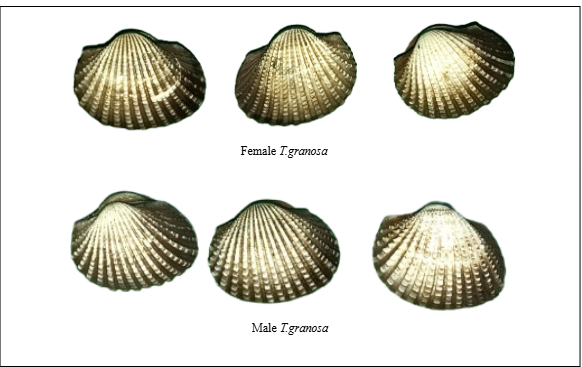
\includegraphics[width=0.9\textwidth]{figures/male-female T.granosa.png}
	\caption{Male and Female \Tegillarcagranosa shells}
\end{figure}

\section{Ethical Considerations}
\label{sec:ethical}

The experiment involving blood cockles will be conducted according to the Animal Research: Reporting of In Vivo Experiments (ARRIVE) guidelines and will be reviewed by the Institutional Animal Care and Use Committee (IACUC) of the University of the Philippines Visayas. 

\section{Creating \textit{T. granosa} Dataset}
\label{sec:dataset}

The experiment began by collecting primary observations for 100 samples of \textit{T. granosa.}. For the actual experimentation, the researchers will collect the original dataset by batch until a sample size of 500  \textit{T. granosa} is reached. Linear measurements were gathered by measuring the width, height, length, rib count, length of the hinge line, and distance between their umbos, organized in the CSV file. This dataset is essential for machine learning model training and testing and determining the baseline for the Convolutional Neural Networks. 


The images were saved in JPG format with a file naming convention of the sample’s sex, the orientation or view of the shell, and its corresponding number out of the total 500 samples. Female \textit{T. granosa} samples will begin with 0 in their file name, and males start with 1. Then, followed by the views captured such as (1) dorsal, (2) ventral, (3) anterior, (4) posterior, (5) left lateral, and (6) right lateral (refer to Figure~\ref{fig:granosa_views}), and lastly, a unique sample number. For example, “010001” will be the file name for the first female sample taken from the dorsal view, and “110001” for the first male sample also taken from the dorsal view. 



\begin{figure}[!htbp]
	\centering
	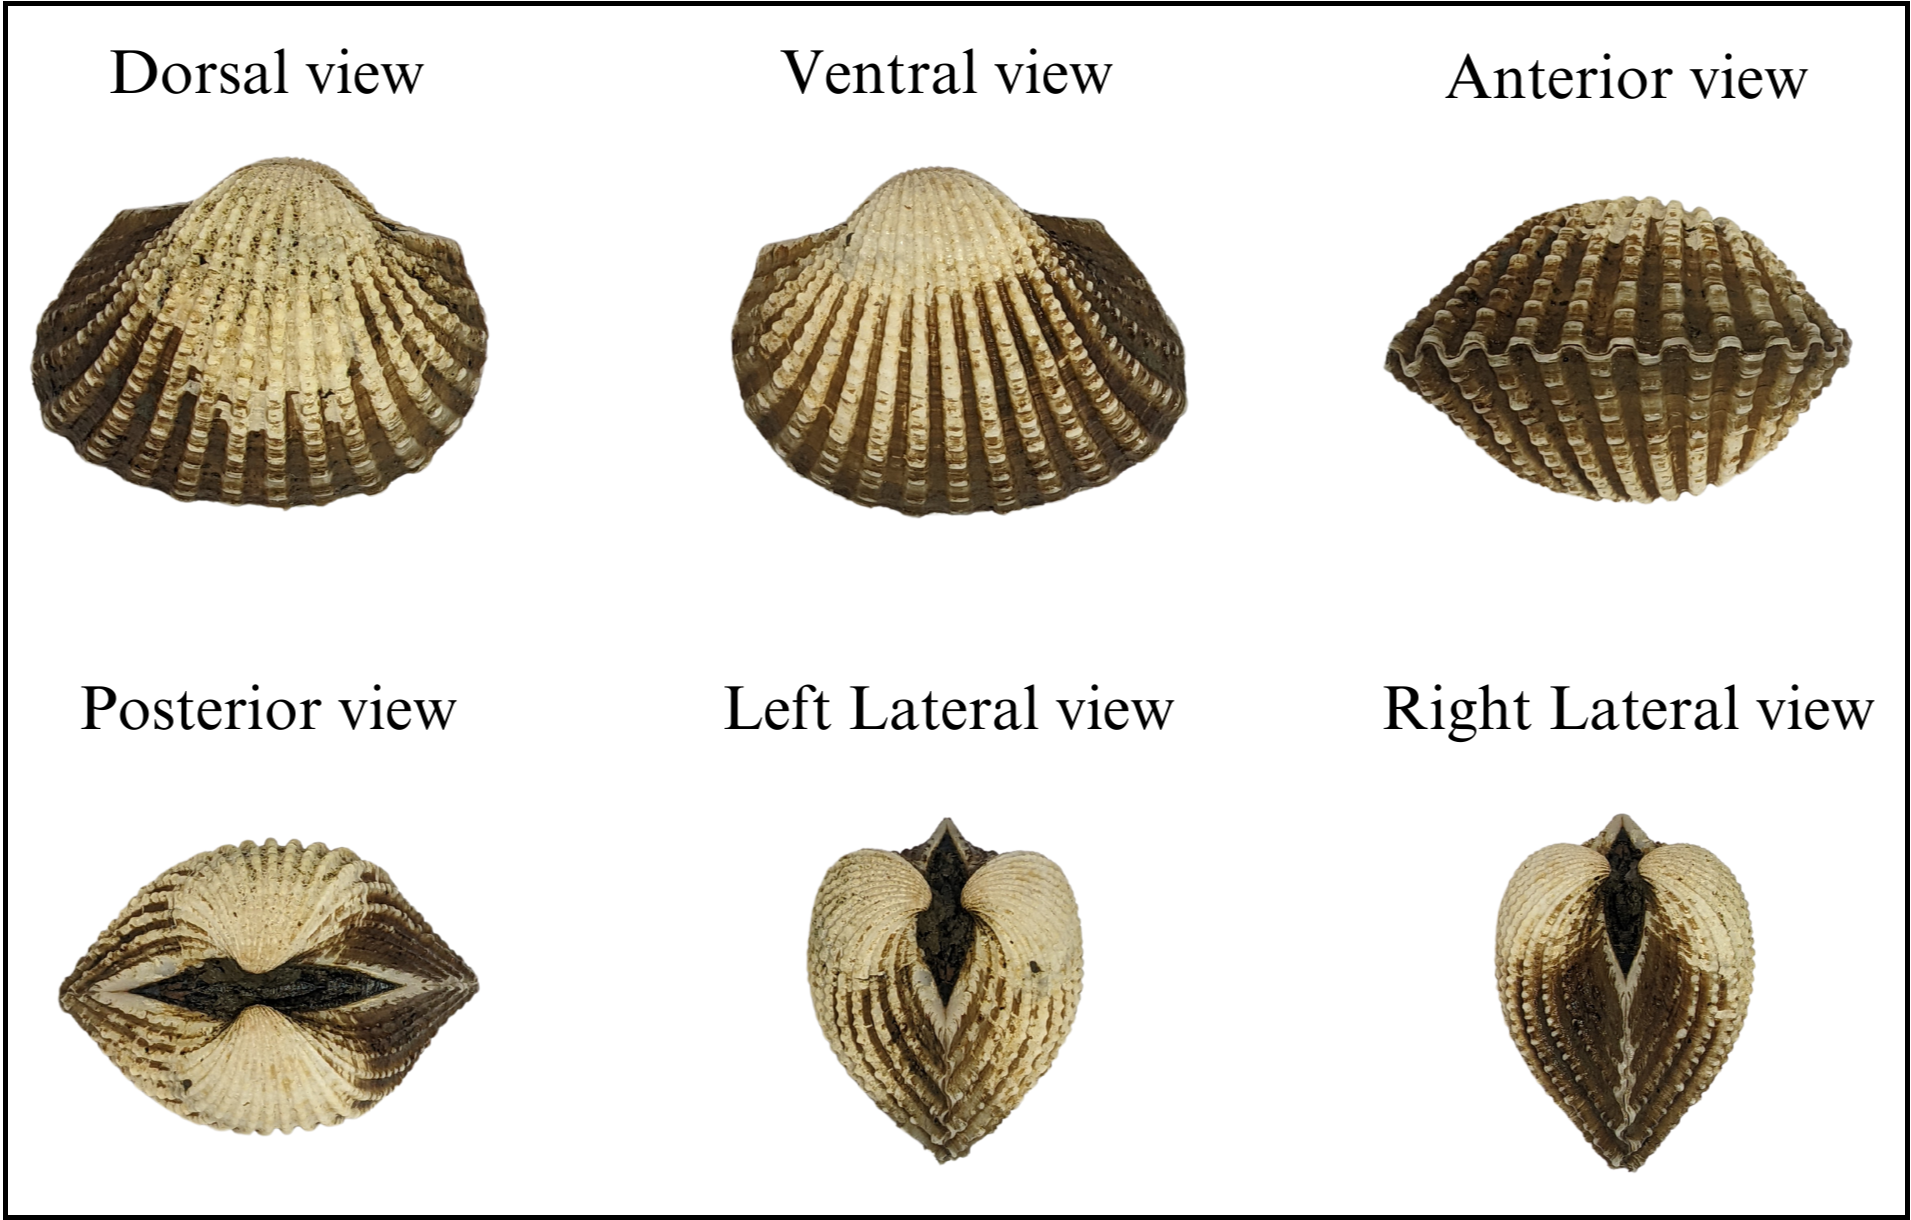
\includegraphics[width=0.9\textwidth]{figures/view.png}
	\caption{Different Views of the \textit{T. granosa} Shell Captured}
	\label{fig:granosa_views}
\end{figure}

\newpage
\section{Morphological and Morphometric Characteristics Collection}
\label{sec:morphochar}

Morphology refers to the biological form and represents one of the most visually recognizable phenotypes across all organisms \cite{tsutsumi2023}. Morphology is a term that describes structural characteristics by measuring specific components, namely, dimensions such as shapes, sizes, and colors. As stated by the researchers, quantifying and characterizing the shape is essential to understanding and visualizing the variations in \textit{T. granosa’s} morphology. 

In this study, the researchers measured the height, width, and length of \textit{T. granosa.} using a Vernier caliper to the nearest 0.01 mm. For the measurements, refer to Figure~\ref{fig:linear_measurements}. The length (A) of the \textit{T. granosa} refers to the measurement from the anterior to the posterior of the shell. The width (B) is the distance across the shell’s widest point from the left to the right valve. The height (C) refers to the measurement from the base of the shell to the shell’s apex. The length of the hinge line (D) near the hinge was measured, along with the distance between the umbos (E). 
Reyment and Kennedy (1998) indicated that incorporating rib count as supplementary information increases identification accuracy. Following this, the researchers recorded the rib count of the male and female \textit{T. granosa}, calculating the ratio since the sizes of the blood cockles vary. 

\begin{figure}[!htbp]
	\centering
	\includegraphics[width=0.95\textwidth]{figures/Tegillarca_granosa_linear_measurements.png}
	\caption{Linear Measurements of  \Tegillarcagranosa shell.}
	\label{fig:linear_measurements}
\end{figure}

\section{Image Acquisition and Pre-Processing}
\label{sec:imageprocess}
This study will comprise 250 male and 250 female \Tgranosa images and will contain 1500 images from different angles. The researchers constructed a box-like structure with a white background surface to control the environment, capturing the images of the samples. This setup aimed to maintain uniform captures of the images, fixing the camera at a consistent angle above the \textit{T. granosa}. A ring light was positioned in front of the box to ensure the image quality, eliminate shadows, and ensure the clarity of the sample during the image acquisition process. Google Pixel 3 XL is the smartphone used with the following specifications: 2960 x 1440 for the resolution, 4,032 x 3,024 pixels (12.2 MP) for the dimensions, f/1.8 for the fstop, 28mm (wide), ½.55”, 1.4µm, dual pixel PDAF, OIS \cite{concepcion2023}

\begin{figure}[!htbp]
	\centering
	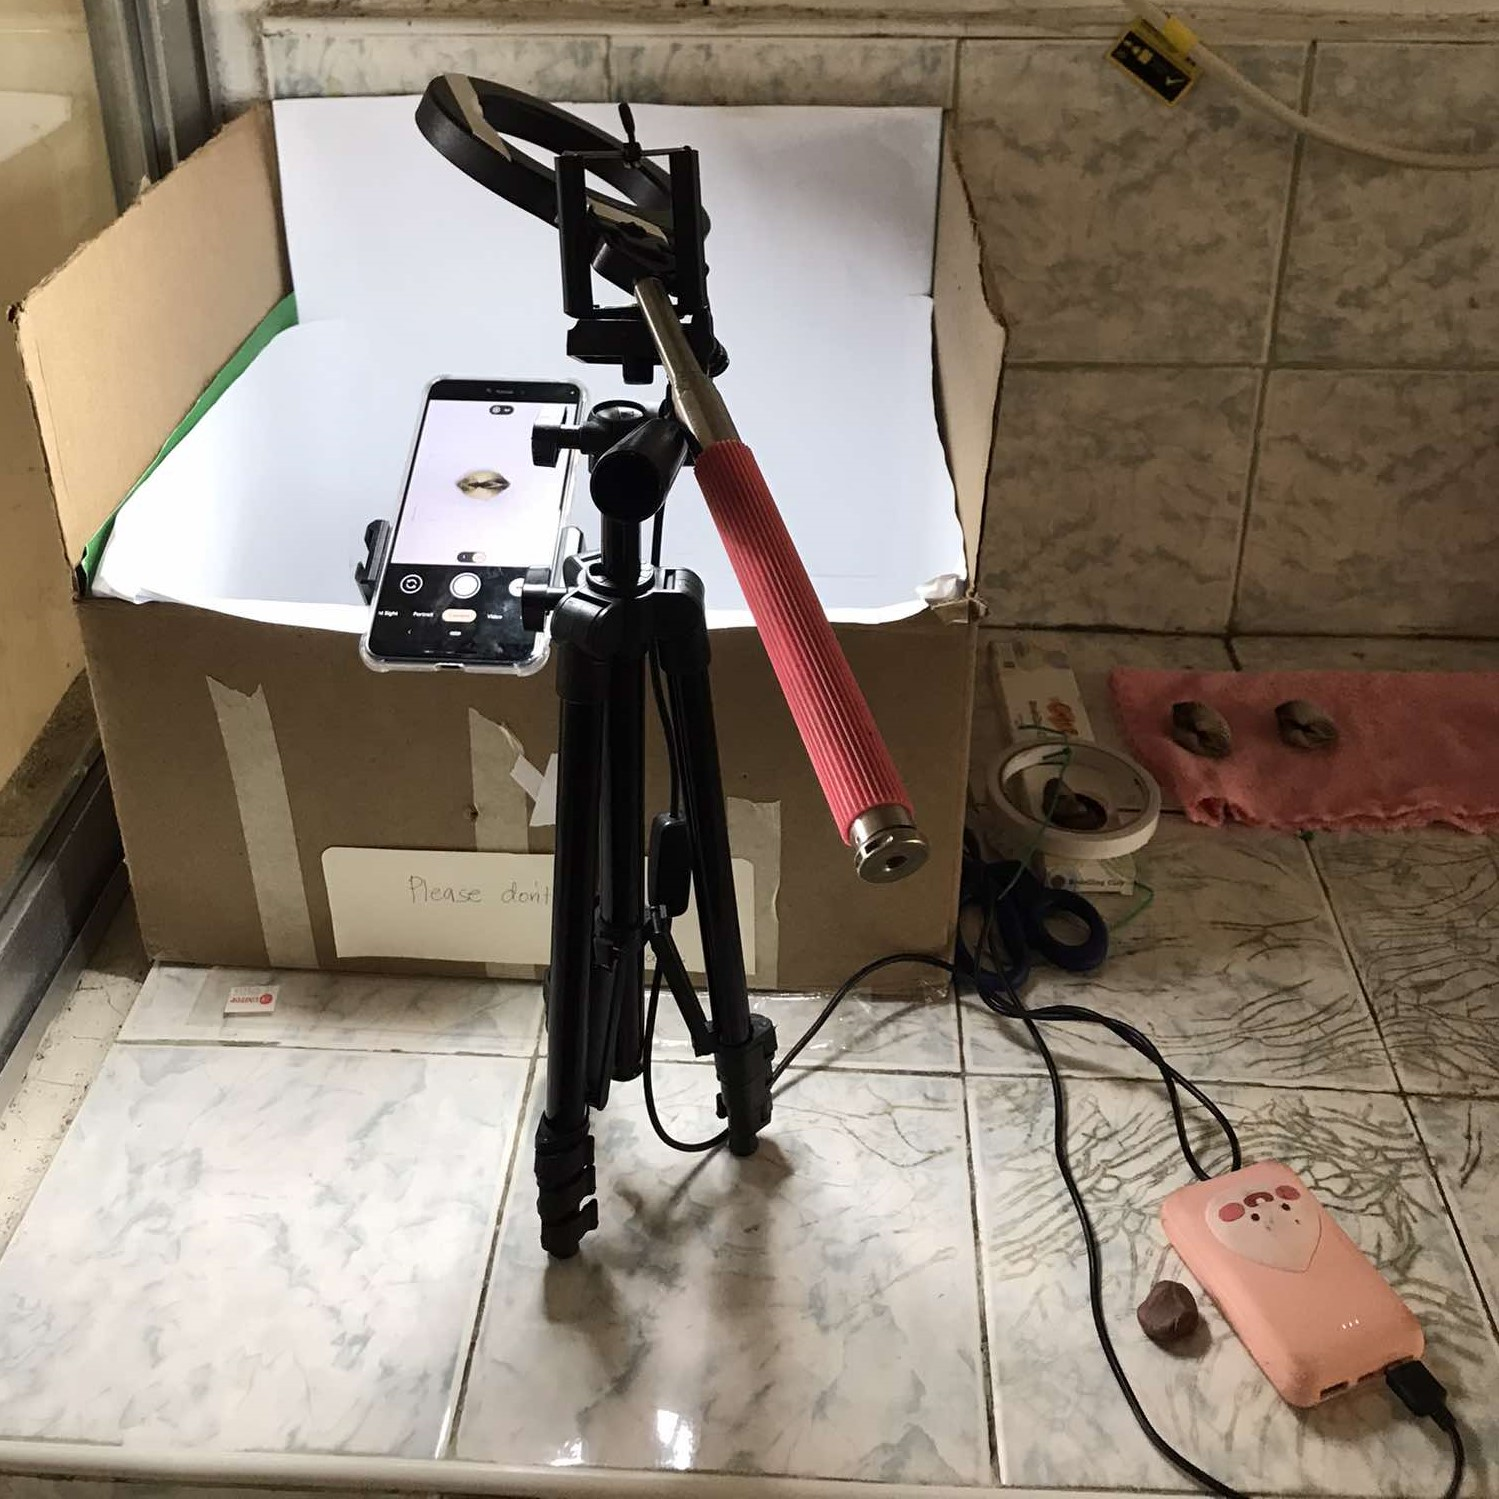
\includegraphics[width=0.4\textwidth]{figures/setup.jpg}
	\caption{Image Acquisition Setup for \textit{T. granosa} Samples}
	\label{fig: setup}
\end{figure}

\section{Hardware and Software Configuration}
This section of the paper discusses the software, programming language, and necessary tools for sex identification. Data collection, preprocessing, and model training were implemented on the Windows 11 operating system using ACER Aspire 3 general processing unit (GPU) with a central processing unit (CPU) of  AMD Ryzen 3 7320U with Radeon Graphics (8) @ 2.395GHz and with a memory of 8 gigabytes (GB). 
Google Collaboratory is utilized for collaborative preprocessing and data visualizations. The results of the gathered measurements were stored and managed in the spreadsheet. GitHub is used for version control, documentation, and tracking activities throughout the study. Python served as the primary programming language used. Lastly, Matlab is used for machine learning operations and training machine learning algorithms. 


\section{Morphometric Characteristics Evaluation Using Machine Learning }
\label{sec:ml models}

This section of the paper discusses the machine-learning operations that serve as a baseline before delving into more complex deep-learning methods for image classification. The study variables collected were linear measurements (length, width, height, length hinge line, distance between umbos, and rib count), along with additional features such as the length-width ratio and the length-height ratio as the features or the predictors. Then, samples are classified by sex (female = 0, male = 1), which serves as the response variable. 

The preprocessing was performed in the Google Collaboratory and involved dropping duplicates, assigning labels, and feature engineering by calculating the ratios. Model training and selection were performed using MatLab Software version 24.2.0.2712019 (R2024b). A cross-fold validation (k = 5), was applied to partition the dataset and estimate accuracy in each fold. The model selection, normalization, model performance, evaluation metrics (accuracy, precision, recall, and F1 score), and other visualizations were also performed on MatLab. 

\subsection{Evaluation Metrics for Machine Learning}
Evaluating the performance of the binary classification model is important as well as selecting the appropriate metrics that is based on the requirements of the user. The performance of the supervised machine learning models will be measured based on three metrics namely: accuracy, precision, recall, and F1 score. 

Accuracy (ACC) is the ratio of the overall correctly predicted samples to the total number of examples in the evaluation dataset \cite{cui2020}. The overall correctness of the model in predicting male and female blood cockles. This metric could help in understanding how well the model performs across all classifications. The formula for the accuracy is: 

\begin{equation}
	\text{PREC} = \frac{\text{Correctly classified samples}} {\text{All samples }} = \frac{TP+ TN}{TP + FP + TN + FN}
	\label{eq:acc}
\end{equation}
Precision (PREC) is the ratio between correctly predicted samples in all samples that are assigned to the positive class \cite{cui2020}. This metric promotes fair representation and prevents the misidentification of blood cockles as it identifies potential inaccuracies or biases. The formula for precision is:


\begin{equation}
	\text{PREC} = \frac{\text{True positive samples}} {\text{Samples assigned to class }} = \frac{TP}{TP + FP}
	\label{eq:prec}
\end{equation}

Recall (REC) is known as the sensitivity or the true positive rate (TPR) which is the ratio of the correctly predicted cases from all the samples assigned to the actual positive cases \cite{cui2020}. This metric is the ability of the model to correctly identify positive male and female samples. The formula for the recall is:

\begin{equation}
	\text{REC} = \frac{\text{True positive samples}} {\text{Samples classified positive}} = \frac{TP}{TP + FN}
	\label{eq:rec}
\end{equation}

F1 score (F1) is defined as the mean of the precision and recall in which it penalizes the extreme values of either of the two \cite{cui2020}. The formula for the F1 is: 

\begin{equation}
	\text{REC} = \frac{ precision \times recall }{precision \times recall }= \frac{2 \times TP}{2 \times TP + FP + FN}
	\label{eq:f1}
\end{equation}

\section{ Deep Learning for Image-Based Classification}
\label{sec:deeplearning}
After collecting a sufficient number of images and identifying initial patterns, convolutional neural networks (CNNs) will be used. CNN has been effectively applied in phenotype classification \cite{kim2024}. In this study, the deep learning model will be specifically adapted for the sex identification of \textit{T. granosa} based on shell images. CNN has achieved breakthroughs in terms of image classification, image segmentation, and speech recognition \cite{he2018}. In this study, CNNs will analyze the images and learn important details about their shapes that can help identify whether they are male or female. Due to the limitation of literature focusing on the sex determining mechanism for bivalves, particularly \textit{T. granosa}. 



